%20 min preso!
\documentclass[xcolor=table]{beamer}
\usepackage{beamerthemesplit}
\usepackage{wrapfig}
\usetheme{SPbGU}
\usepackage{pdfpages}
\usepackage{amsmath}
\usepackage{cmap}
\usepackage[T2A]{fontenc}
\usepackage[utf8]{inputenc}
\usepackage[english]{babel}
\usepackage{indentfirst}
\usepackage{amsmath}
\usepackage{tikz}
\usetikzlibrary{automata,positioning}
\usepackage{multirow}
\usepackage[noend]{algpseudocode}
\usepackage{algorithm}
\usepackage{algorithmicx}
\usepackage{fancyvrb}
\usepackage{subcaption}
\usepackage{listings}
%\usepackage{multicol}
\usetikzlibrary{calc}
\usetikzlibrary{shapes,arrows}
\usetikzlibrary{arrows,automata}
\usetikzlibrary{positioning}

\usepackage{tabularx}
\newcolumntype{Y}{>{\raggedleft\arraybackslash}X}


\newtheorem{mytheorem}{Theorem}
\renewcommand{\thealgorithm}{}

\newcommand{\tikzmark}[1]{\tikz[overlay,remember picture] \node (#1) {};}
\def\Put(#1,#2)#3{\leavevmode\makebox(0,0){\put(#1,#2){#3}}}

\tikzset{
    state/.style={
           rectangle,
           rounded corners,
           draw=black, very thick,
           minimum height=2em,
           inner sep=2pt,
           text centered,
           },
    horiz/.style={
                  % font=\tiny,
              inner sep=3pt,
              font=\bf

                  } ,
    point/.style={
                  circle,
                  minimum width = 5pt,
                  fill
                  },
}




\beamertemplatenavigationsymbolsempty

\title[Parsing Techniques for CFPQ]{Parsing Techniques for Contex-Free Path Querying}
%\subtitle[YaccConstructor]{Parsing techniques for graph analysis}
% То, что в квадратных скобках, отображается в левом нижнем углу.
\institute[JetBrains Research]{
JetBrains Research, Programming Languages and Tools Lab  \\
Saint Petersburg University
}

% То, что в квадратных скобках, отображается в левом нижнем углу.
\author[Semyon Grigorev]{\textbf{Semyon Grigorev}}

\date{April 05, 2019}

\begin{document}
{
\begin{frame}[fragile]
%  \begin{table}
%  \centering
%  \begin{tabularx}{\linewidth}{YcX}
%    
\includegraphics[height=1.5cm]{pictures/jetbrainsResearch.pdf} \hfill
%    & \begin{minipage}[t]{0.3\textwidth}\center \vspace{-1cm}
%      \end{minipage}
%    & \hfill \includegraphics[height=1.5cm]{pictures/SPbGU_Logo.png}
%  \end{tabularx}
%  \end{table}
  \titlepage
\end{frame}
}

%\begin{frame} \frametitle{Programming Languages and Tools Lab}
%    \begin{itemize}
%      \item \url{https://research.jetbrains.org/groups/plt_lab}
%    \end{itemize}
%\end{frame}




\begin{frame} \frametitle{Formal language constrained path querying}
\begin{itemize}
\item Finite directed edge-laballed graph $\mathcal{G} = (V,E,L)$
\item The path is a world over $L$: $\omega(p) = \omega(v_0 \xrightarrow{l_0} v_1 \xrightarrow{l_1} \dots \xrightarrow{l_{n-1}} v_n ) = l_0 \cdot l_1 \cdot \ldots \cdot l_{n-1}$
\item The language $\mathcal{L}$ (over $L$)
\end{itemize}
\pause
\begin{itemize}
  \item Reachability problem: $Q=\{(v_i,v_j) \ | \ \exists p = v_i \dots v_j, \omega(p) \in \mathcal{L}\}$
  \item Path querying problem: $Q=\{p \ | \ \omega(p) \in \mathcal{L}\}$
  \begin{itemize}
    \item Single path, all paths, shortest path \dots
  \end{itemize}
\end{itemize}

\end{frame}

\begin{frame} \frametitle{Context-Free path querying}
\begin{itemize}
\item $\mathcal{L}$ is a context-free language
\item $G_{\mathcal{L}} = (N,\Sigma,R,S)$
\item Reachability problem: $Q=\{(v_i,v_j) \ | \ \exists p = v_i \dots v_j, S \xrightarrow[G_L]{*} \omega(p) \}$
\item Path querying problem: $Q=\{p \ | \ \omega(p) \in \mathcal{L}\}$
\end{itemize}

\end{frame}

\begin{frame} \frametitle{Example of CFPQ}

\begin{center}
  \begin{tabular}{  c  c  }
      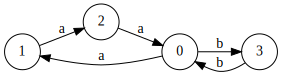
\includegraphics[width=0.45\textwidth]{pictures/input.pdf}
      &
  $

  \begin{array}{rl}
     0:& S \rightarrow a \ S \ b \\
     1:& S \rightarrow Middle \\
     2:& Middle \rightarrow a \ b
  \end{array}

  $
  \\
  Input graph
  &
  Query: language $\{a^nb^n \ | \ n > 0 \}$

  \end{tabular}
\end{center}
\vspace{0.5cm}
Paths: \\
$2 \xrightarrow{a} 0 \xrightarrow{b} 3$ \\
$1 \xrightarrow{a} 2 \xrightarrow{a} 0 \xrightarrow{b} 3 \xrightarrow{b} 0$ \\
$p_1 = 0 \xrightarrow{a} 1 \xrightarrow{a} 2 \xrightarrow{a} 0 \xrightarrow{b} 3 \xrightarrow{b} 0 \xrightarrow{b} 3$ \\
$p_2 = 0 \xrightarrow{a} 1 \xrightarrow{a} 2 \xrightarrow{a} 0 \xrightarrow{a} 1 \xrightarrow{a} 2 \xrightarrow{a} 0 \xrightarrow{b} 3 \xrightarrow{b} 0 \xrightarrow{b} 3 \xrightarrow{b} 0 \xrightarrow{b} 3 \xrightarrow{b} 0$ \\
$\dots$

\end{frame}


\begin{frame} \frametitle{Applications}
\begin{itemize}
\item Graph data bases querying \\
Yann ...
\item Static code analysis \\
Reps CFL reachability
\item CFL editing distance/Error recovery \\
Aho
\end{itemize}
\end{frame}

\begin{frame} \frametitle{Graph data bases querying}

\begin{minipage}[t]{0.5\textwidth}
\begin{tikzpicture}[shorten >=1pt, >=stealth', node distance=1.5cm,on grid,auto]
   \node[state] (0) {July};
   \node[state] (1) [below left=of 0]  {Mark};
   \node[state] (2) [below right=of 0] {Anna};
   \node[state] (3) [below=of 1]  {Steve};
   \node[state, blue] (4) [below=of 2] {You};
   \node[state, red] (5) [below left=of 3]  {John};
   \node[state, red] (6) [below right=of 5, right=of 5] {Alice};
   \node[state] (7) [below=of 4, right=of 6] {Will};
   \node[state] (8) [below=of 4, right=of 7] {Lisa};

   \path[->]
%    (0) edge[horiz] node[sloped, above] {child} (1)
    (0) edge node        {} (2)
    (0) edge node        {} (1)
    (1) edge node        {} (3)
    (3) edge node        {} (5)
    (3) edge node        {} (6)
    (2) edge node        {} (4)
    (4) edge node        {} (7)
    (4) edge node        {} (8)
       ;
\end{tikzpicture}
\end{minipage}
~
\begin{minipage}[t]{0.45\textwidth}
\vspace{-3cm}
Find your cousins once removed
\begin{align*}
S& \rightarrow H \boldsymbol{\downarrow}  \\
H& \rightarrow \varepsilon \mid  \, \boldsymbol{\uparrow} \, H \, \boldsymbol{\downarrow}
\end{align*}
\end{minipage}

\vspace{1cm}
Same generation query, similarity query.


\end{frame}


\begin{frame}[fragile] \frametitle{Static code analysis}
  \begin{minipage}[t]{0.45\textwidth}
    \vspace{-7.5cm}
    \lstset{language=C,basicstyle=\small}
    \begin{lstlisting}
    int id(int u)
    {
      v = u;
      return v;
    }
    int main()
    {
      //taint
      int x;
      int z, y;
      //untaint
      int t;
      z = id(x);
      t = id(y);
    }
  \end{lstlisting}
\end{minipage}
~
\begin{minipage}[t]{0.45\textwidth}
  \begin{tikzpicture}[shorten >=1pt, >=stealth', node distance=1.9cm,on grid,auto]
  \tikzstyle{none} = [draw=none, minimum height=0.4cm, minimum width=1cm]
     \node[none]  (a)              {\emph{taint}};
     \node[state] (b) [below of=a] {$x$};
     \node[state] (d) [below of=b] {$u$};
     \node[state] (c) [below of=d] {$y$};
     \node[state] (e) [right of=d] {$v$};
     \node[state] (f) [above of=e] {$z$};
     \node[state] (g) [below of=e] {$t$};
     \node[none]  (h) [below of=g] {\emph{untaint}};
     \path[->]
      (a) edge[horiz] node[left]  {save} (b)
      (b) edge[horiz] node[left]  {$\boldsymbol{call\_id}_1$} (d)
      (c) edge[horiz] node        {$\boldsymbol{call\_id}_2$} (d)
      (d) edge[horiz] node        {save} (e)
      (e) edge[horiz] node[right] {$\boldsymbol{ret\_id}_1$} (f)
      (e) edge[horiz] node        {$\boldsymbol{ret\_id}_2$} (g)
      (g) edge[horiz] node        {save} (h)

      ;
  \end{tikzpicture}

\end{minipage}

\end{frame}

\begin{frame} \frametitle{Error recovery}
\begin{itemize}
\item !!!!
\end{itemize}
\end{frame}

\begin{frame}[fragile]
  %\transwipe[direction=90]
  \frametitle{Structural representation of result}
  \begin{center}
    \begin{tabular}{  c  c  }
        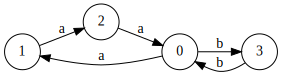
\includegraphics[width=0.45\textwidth]{pictures/input.pdf}
        &
    $

    \begin{array}{rl}
       0:& S \rightarrow a \ S \ b \\
       1:& S \rightarrow Middle \\
       2:& Middle \rightarrow a \ b
    \end{array}

    $
    \\
    Input graph
    &
    Grammar

    \end{tabular}
  \end{center}

\begin{tabular}{  c  c  c  }
      \onslide<2-4>{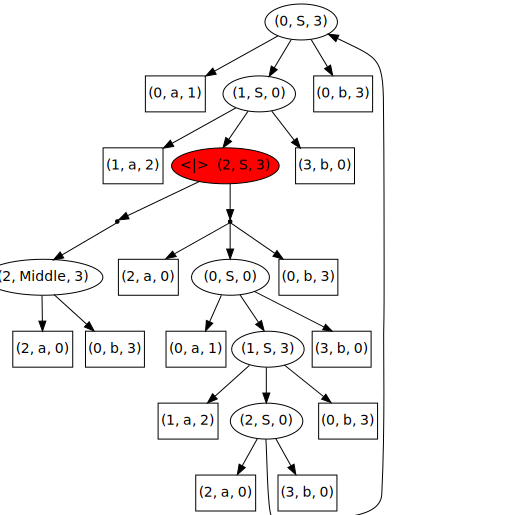
\includegraphics[height=4.5cm]{pictures/AnBn.pdf}}
    &
      \onslide<3-4>{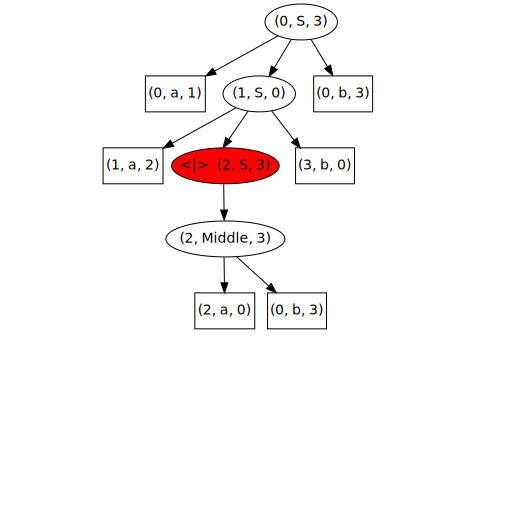
\includegraphics[height=4.5cm]{pictures/AnBn_2.pdf}}
    &
      \onslide<4>{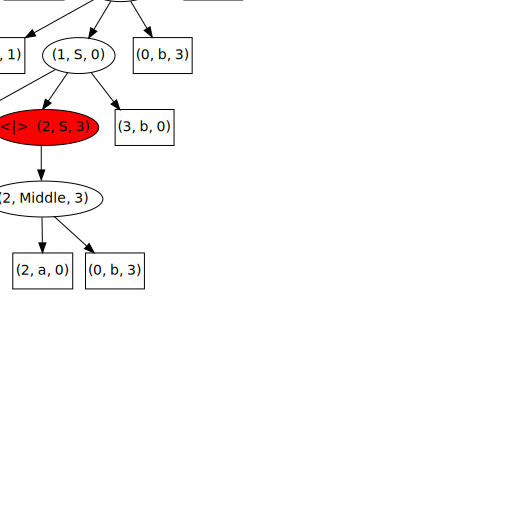
\includegraphics[height=4.5cm]{pictures/AnBn_1.pdf}}

\\
\onslide<2-4>{\small{Query result (SPPF)}}
& \onslide<3-4>{\small{Tree for $p_1$}}
& \onslide<4>{\small{Tree for $p_2$}}
  \end{tabular}
%\end{center}
\end{frame}

\begin{frame}[fragile] \frametitle{Paths extraction}
\begin{center}
\begin{tabular}{  c  c  }
    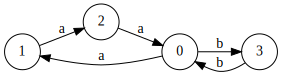
\includegraphics[width=0.45\textwidth]{pictures/input.pdf}
    &
$

\begin{array}{rl}
   0:& S \rightarrow a \ S \ b \\
   1:& S \rightarrow Middle \\
   2:& Middle \rightarrow a \ b
\end{array}

$
\end{tabular}

\begin{figure}[ht]
    \centering
        \includegraphics[width=0.68\textwidth]{pictures/AnBn_2_m.pdf}
\end{figure}
Path: $0\xrightarrow{a}1\xrightarrow{a}2\xrightarrow{a}0\xrightarrow{b}3\xrightarrow{b}0\xrightarrow{b}3$
\end{center}
\end{frame}


\begin{frame}[fragile]
  %\transwipe[direction=90]
  \frametitle{Bar-Hillel theorem}
Context-free languages are closed under intersection with regular languages
\begin{center}
\begin{tabular}{  c  c  }
    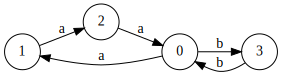
\includegraphics[width=0.35\textwidth]{pictures/input.pdf}
    &
$

\begin{array}{rl}
   0:& S \rightarrow a \ S \ b \\
   1:& S \rightarrow Middle \\
   2:& Middle \rightarrow a \ b
\end{array}

$
\\
Regular language
&
Context-free language

\end{tabular}

\vspace{0.8em}
\pause

\begin{tabular}{  c  c  }
    \raisebox{-0.5\totalheight}{\includegraphics[width=0.32\textwidth]{pictures/AnBn_m.pdf}}
    &
\pause
$
\begin{array}{rl}
   (0,S,3) & \rightarrow (0,a,1) \ (1,S,0) \ (0,b,3) \\
   (1,S,0) & \rightarrow (1,a,2) \ (2,S,3) \ (3,b,0) \\
   (2,S,3) & \rightarrow (2,a,0) \ (0,S,0) \ (0,b,3) \\
   (2,S,3) & \rightarrow (2,Middle,3)                \\
   (0,S,0) & \rightarrow (0,a,1) \ (1,S,3) \ (3,b,0) \\
   (1,S,3) & \rightarrow (1,a,2) \ (2,S,0) \ (0,b,3) \\
   (2,S,0) & \rightarrow (2,a,0) \ (0,S,3) \ (3,b,0) \\
   (0,Middle,3) & \rightarrow (2,a,0) \ (0,b,3)  \\
\end{array}
$

\end{tabular}
\end{center}
\end{frame}


\begin{frame} \frametitle{Directions for research}
\begin{itemize}
\item Parallel and distributed parsing
\item O(BMM) complexity
\item Incremental parsing
\end{itemize}
\end{frame}


\begin{frame}
\frametitle{Contact Information}
\begin{itemize}
  \item Semyon Grigorev:
    \begin{itemize}
      \item \href{mailto:s.v.grigoriev@spbu.ru}{s.v.grigoriev@spbu.ru}
      \item \href{mailto:Semen.Grigorev@jetbrains.com}{Semen.Grigorev@jetbrains.com}
    \end{itemize}

\end{itemize}

\end{frame}

\end{document}
